\documentclass[tikz,border=8pt]{standalone}
\usetikzlibrary{arrows.meta,positioning,fit,calc}
\begin{document}
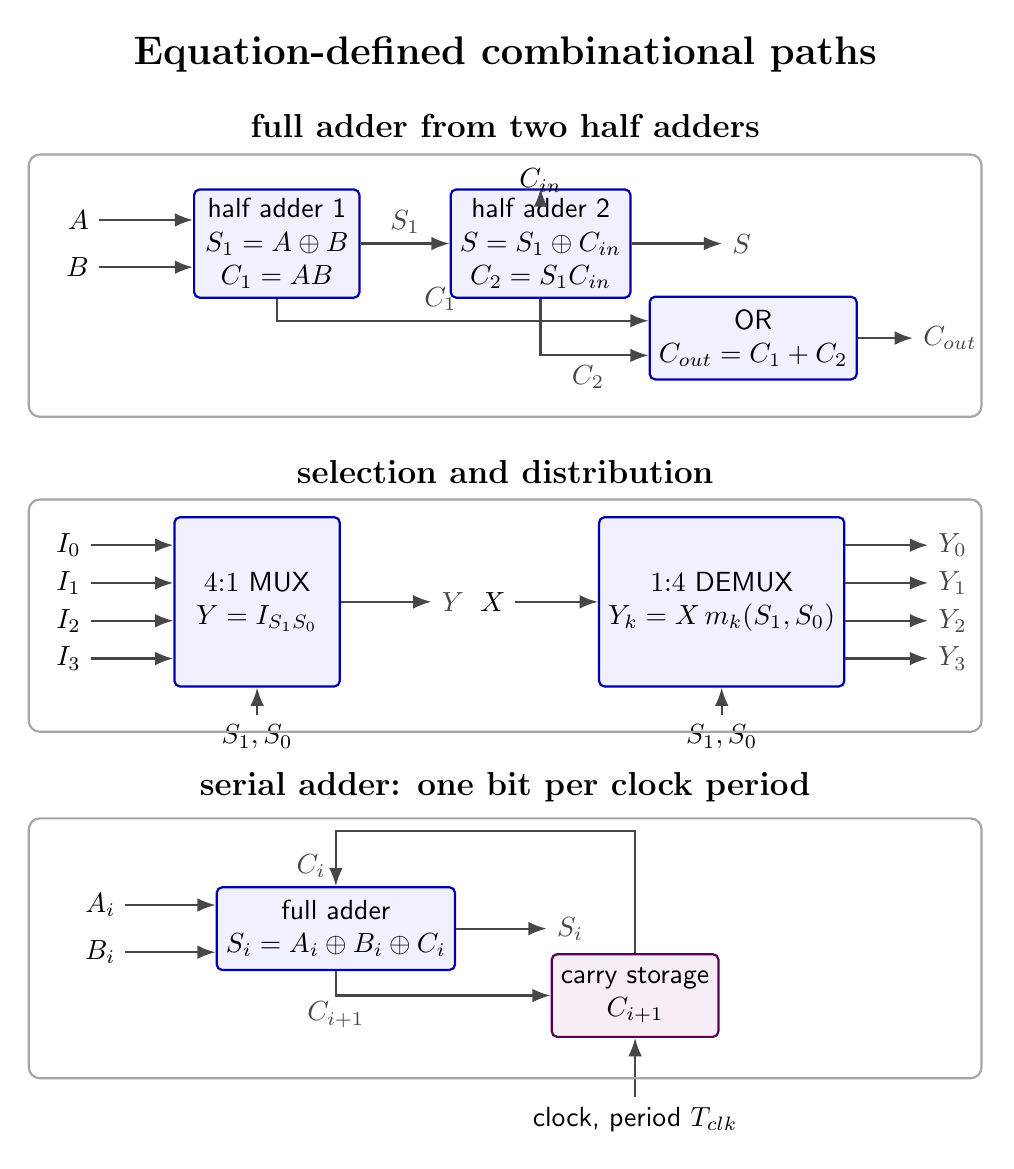
\begin{tikzpicture}[
  font=\sffamily,
  >=Latex,
  block/.style={draw=blue!65!black,rounded corners=2pt,thick,minimum width=2.1cm,minimum height=1.05cm,align=center,fill=blue!6},
  state/.style={block,draw=violet!70!black,fill=violet!7},
  line/.style={->,thick,black!72},
  frame/.style={draw=black!35,rounded corners=4pt,thick}
]
\node[font=\bfseries\Large] at (6.6,13.05) {Equation-defined combinational paths};

% Full adder from two half adders.
\node[font=\bfseries\large] at (6.6,12.15) {full adder from two half adders};
\node[block] (ha1) at (3.7,10.65) {half adder 1\\$S_1=A\oplus B$\\$C_1=AB$};
\node[block] (ha2) at (7.05,10.65) {half adder 2\\$S=S_1\oplus C_{in}$\\$C_2=S_1C_{in}$};
\node[block,minimum width=1.45cm] (org) at (9.75,9.45) {OR\\$C_{out}=C_1+C_2$};
\node[left=1.2cm of ha1,yshift=.3cm] (a) {$A$};
\node[left=1.2cm of ha1,yshift=-.3cm] (b) {$B$};
\draw[line] (a) -- ([yshift=.3cm]ha1.west);
\draw[line] (b) -- ([yshift=-.3cm]ha1.west);
\draw[line] (ha1.east) -- node[above] {$S_1$} (ha2.west);
\node (ci) at (7.05,11.45) {$C_{in}$};
\draw[line] (ci) -- (ha2.north);
\draw[line] (ha2.east) -- ++(1.15,0) node[right] {$S$};
\draw[line] (ha1.south) |- node[pos=.72,above] {$C_1$} ([yshift=.22cm]org.west);
\draw[line] (ha2.south) |- node[pos=.72,below] {$C_2$} ([yshift=-.22cm]org.west);
\draw[line] (org.east) -- ++(.7,0) node[right] {$C_{out}$};
\draw[frame] (.55,8.45) rectangle (12.65,11.78);

% Multiplexer and demultiplexer.
\node[font=\bfseries\large] at (6.6,7.75) {selection and distribution};
\node[block,minimum height=2.15cm] (mux) at (3.45,6.1) {$4{:}1$ MUX\\$Y=I_{S_1S_0}$};
\foreach \i/\dy in {0/.72,1/.24,2/-.24,3/-.72}{
  \node[left=1.05cm of mux,yshift=\dy cm] (i\i) {$I_\i$};
  \draw[line] (i\i) -- ([yshift=\dy cm]mux.west);
}
\node[below=.35cm of mux] (selm) {$S_1,S_0$};
\draw[line] (selm) -- (mux.south);
\draw[line] (mux.east) -- ++(1.15,0) node[right] {$Y$};

\node[block,minimum height=2.15cm] (demux) at (9.35,6.1) {$1{:}4$ DEMUX\\$Y_k=X\,m_k(S_1,S_0)$};
\node[left=1.05cm of demux] (xin) {$X$};
\draw[line] (xin) -- (demux.west);
\node[below=.35cm of demux] (seld) {$S_1,S_0$};
\draw[line] (seld) -- (demux.south);
\foreach \i/\dy in {0/.72,1/.24,2/-.24,3/-.72}{
  \draw[line] ([yshift=\dy cm]demux.east) -- ++(1.05,0) node[right] {$Y_\i$};
}
\draw[frame] (.55,4.45) rectangle (12.65,7.4);

% Serial adder: only carry is stored between clock periods.
\node[font=\bfseries\large] at (6.6,3.75) {serial adder: one bit per clock period};
\node[block] (fa) at (4.45,1.95) {full adder\\$S_i=A_i\oplus B_i\oplus C_i$};
\node[state] (ff) at (8.25,1.1) {carry storage\\$C_{i+1}$};
\node[left=1.15cm of fa,yshift=.3cm] (ai) {$A_i$};
\node[left=1.15cm of fa,yshift=-.3cm] (bi) {$B_i$};
\draw[line] (ai) -- ([yshift=.3cm]fa.west);
\draw[line] (bi) -- ([yshift=-.3cm]fa.west);
\draw[line] (fa.east) -- ++(1.15,0) node[right] {$S_i$};
\draw[line] (fa.south) |- node[pos=.42,below] {$C_{i+1}$} (ff.west);
\draw[line] (ff.north) |- ++(-1.0,1.55) -| node[pos=.82,left] {$C_i$} (fa.north);
\node[below=.75cm of ff] (clk) {clock, period $T_{clk}$};
\draw[line] (clk) -- (ff.south);
\draw[frame] (.55,.05) rectangle (12.65,3.35);
\end{tikzpicture}
\end{document}
